\section{Robustness of the verdicts}
\label{sec:validation}

Every verdict comes from one pre-registered rule applied to five paired seeds. This
section asks how much the verdicts on the six-problem matrix depend on that rule and on
individual seeds. All of it is computed from the committed runs
(\texttt{scripts/report/fig\_validation.py}); no model was retrained.

\paragraph{Bootstrap intervals.} Figure~\ref{fig:bootstrap} resamples the five paired
seeds 5{,}000 times and gives a 95\% interval for each pre-registered error ratio. The
heat design-versus-random result is robust: the designed circuit's error is 6.5$\times$
lower, with the whole interval (2.5$\times$ to 17.7$\times$) above the 1.5$\times$ bar. The
one-copy Poisson comparisons against classical models fail decisively rather than
narrowly: against the MLP the interval is 0.40 to 1.10 (bar 2$\times$), against Fourier
features 0.01 to 0.43, and against the frequency-matched model 3.9 to 5.8, entirely
outside its equivalence band. The one-copy Poisson design-versus-random ratio (1.84,
interval 0.97 to 7.2) straddles its threshold, as an inconclusive verdict should.

\paragraph{Other tests.} With five paired seeds the smallest two-sided Wilcoxon $p$ is
$1/16=0.0625$ however large the effect, so the confirmation rule can only be met by five
seeds of five agreeing. Three alternative tests on the same pairs agree with every
verdict and show what the Wilcoxon floor hides: on the heat design-versus-random
comparison a paired $t$-test on log error gives $p=0.006$ and a Mann--Whitney test
$p=0.008$.

\paragraph{Leave one seed out.} If one seed decided a verdict, dropping it would move
the ratio across its threshold. With each seed removed in turn, the heat
design-versus-random ratio clears its bar all five times, the one-copy Poisson
comparisons against classical models miss theirs all five times, and the one-copy Poisson
design-versus-random ratio clears it four times of five. No verdict rests on a single
seed.

\begin{figure}[htbp]
  \centering
  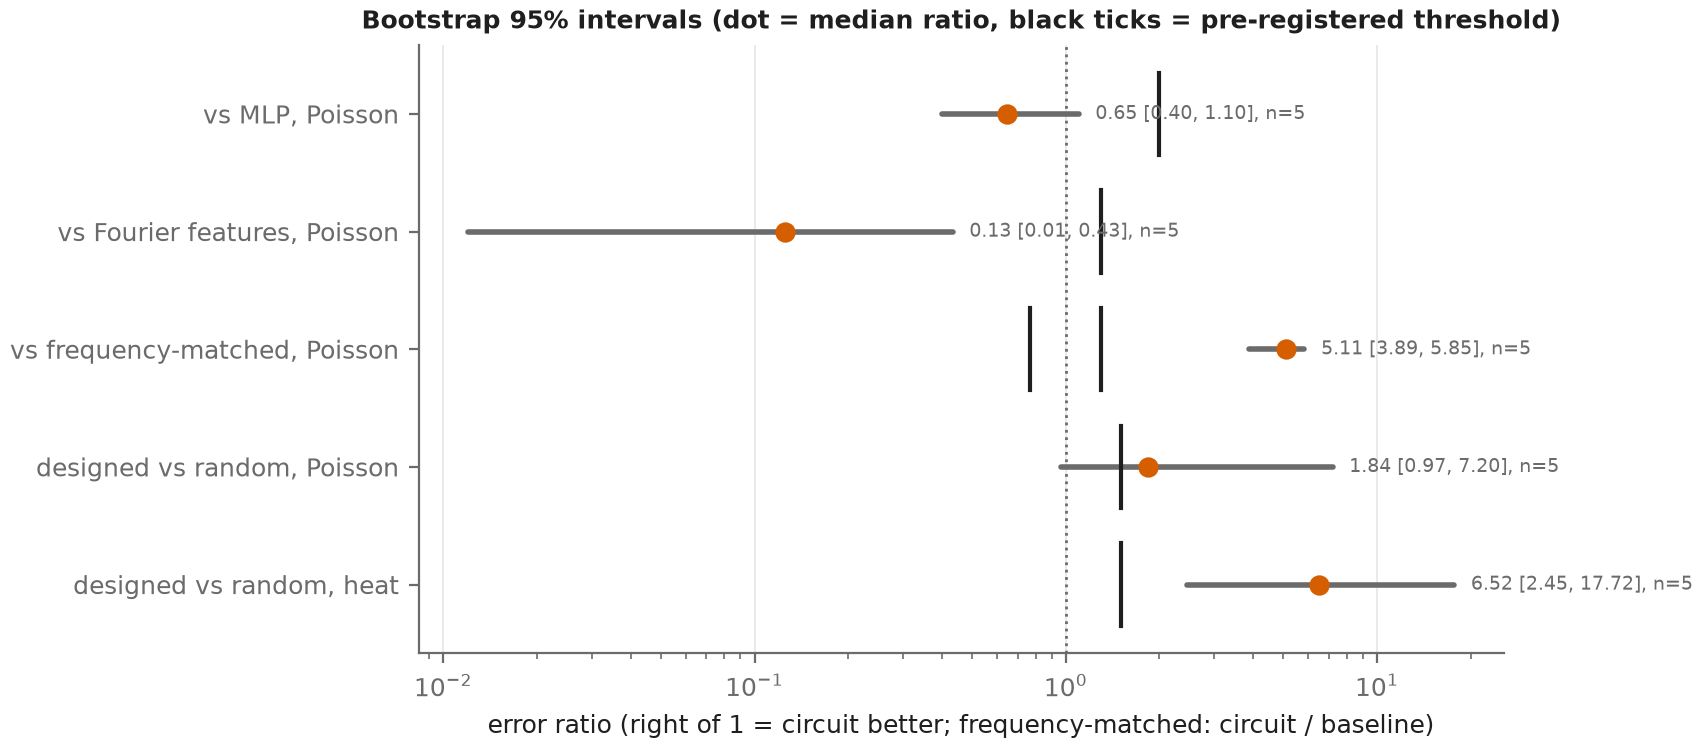
\includegraphics[width=0.65\linewidth]{../results/report/figures/validation_bootstrap_ratios.png}
  \caption{Bootstrap 95\% intervals of the pre-registered error ratios, one copy of the
    circuit (5 paired seeds, 5{,}000 resamples). Right of 1 means the circuit is better;
    for the frequency-matched comparison the ratio is circuit over baseline and must lie
    between the two ticks.}
  \label{fig:bootstrap}
\end{figure}
